\documentclass{article} 
\usepackage{graphicx}
\usepackage{amssymb}
\usepackage{listings}
\usepackage{MnSymbol}
\usepackage{pgfgantt}
\usepackage{titlesec}
\newcommand{\sectionbreak}{\clearpage}

\lstset{frame=tb,
  language=Java,
  aboveskip=3mm,	
  belowskip=3mm,
  showstringspaces=false,
  columns=flexible,
  basicstyle={\small\ttfamily},
  numbers=none,
  breaklines=true,
  breakatwhitespace=true
  tabsize=3
}


\newtheorem{theorem}{Theorem}[section]
\newtheorem{lemma}[theorem]{Lemma}
\newtheorem{proposition}[theorem]{Proposition}
\newtheorem{corollary}[theorem]{Corollary}

\newenvironment{proof}[1][Proof]{\begin{trivlist}
\item[\hskip \labelsep {\bfseries #1}]}{\end{trivlist}}
\newenvironment{definition}[1][Definition]{\begin{trivlist}
\item[\hskip \labelsep {\bfseries #1}]}{\end{trivlist}}
\newenvironment{example}[1][Example]{\begin{trivlist}
\item[\hskip \labelsep {\bfseries #1}]}{\end{trivlist}}
\newenvironment{remark}[1][Remark]{\begin{trivlist}
\item[\hskip \labelsep {\bfseries #1}]}{\end{trivlist}}



\newcommand{\qed}{\nobreak \ifvmode \relax \else
      \ifdim\lastskip<1.5em \hskip-\lastskip
      \hskip1.5em plus0em minus0.5em \fi \nobreak
      \vrule height0.75em width0.5em depth0.25em\fi}
\newcommand{\pre}{\mathop{\mathrm{pre}}}
\newcommand{\myparagraph}[1]{\paragraph{#1}\mbox{}\\}


\setlength\parindent{6pt}
\setlength{\parskip}{0.4cm}


\newcommand{\HRule}{\rule{\linewidth}{0.5mm}}

\begin{document} 
\begin{titlepage}
\begin{center}

% Upper part of the page. The '~' is needed because \\
% only works if a paragraph has started.

\textsc{\LARGE Imperial College London}\\[1.5cm]

\textsc{\Large Interim Report}\\[0.5cm]

% Title
\HRule \\[0.4cm]
{ \huge \bfseries A Model Checker Based on Sentential Decision Diagrams \\[0.4cm] }

\HRule \\[1.5cm]

% Author and supervisor
\begin{minipage}{0.4\textwidth}
\begin{flushleft} \large
\emph{Author:}\\
Hugo \textsc{Paquet}
\end{flushleft}
\end{minipage}
\begin{minipage}{0.4\textwidth}
\begin{flushright} \large
\emph{Supervisor:} \\
Prof.~Alessio\textsc{ Lomuscio}
\end{flushright}
\end{minipage}

\vfill

% Bottom of the page
{\large \today}

\end{center}
\end{titlepage}

 \tableofcontents 
\clearpage
\section{Intro and Motivation}

\subsection{The Problem}

Autonomous systems are becoming increasingly important in today's world and often their verification is essential to avoid damage and/or profit loss.  Some recent software bugs have had a huge impact, such as the self-destruction of rocket Arianne V and the recall of 400,000 Toyota Prius cars.
The increasing use of safety-critical systems has seen verification of autonomous systems develop into an active aera of research in the past two decades. 

Model checking is an automatic verification technique based on formal methods which allows us to check that a system $S$ possesses a property $P$.  A large amount of research work has been done into verifying larger systems, and recently a variety of techniques have been developed. One of these, \emph{symbolic} model checking, involves representing states and transitions of the model by Boolean functions.

In this project we explore the use of a novel representation of Boolean functions, the Sentential Decision Diagram (SDD) in symbolic model checking. One of the goals of the project is to implement this in MCMAS, a model checker for multi-agent systems. 

\subsection{Report}

In this report, we start with some theory about the temporal and epistemics logics used in the verification of autonomous systems, a review of model checking and the different representations of Boolean functions. Then, we explain in details what SDDs are and present a few elementary results (Chapter 2).

 In view of the implementation of a new model checker, we outline a plan of work, giving an overview of the tools and software which will be used (Chapter 3).
 
 Finally, we suggest a few ideas for evaluating the efficiency of the created model checker throughout, and at the end of its implementation (Chapter 4).

\begin{remark}
Due to a lack of writing time, some of the sections in this report are incomplete. In particular, I would have liked to include a more detailed time plan, more concrete examples and some diagrams. 
\end{remark}

\clearpage
\section{Background}

\subsection{Multi-Agent Systems}

Autonomous Multi-Agent Systems (MAS) are computer systems which are made up of several ``agents" acting within an ``environment". 
An \textit{agent} is: 
\begin{itemize}
\item Capable of \textit{autonomous} action 
\item Capable of \textit{social} interaction with peers
\item Acting to \textit{meet} their design objectives 
\end{itemize}
 
Suppose we have an MAS consisting of a set of agents $A = {1, ..., n}$ and an environment $e$.
\begin{definition} 
An agent $i$ in the system consists of: 
\begin{itemize}
\item A set $L_i$ of local states representing the different configurations of the agent
\item A set $Act_i$ of local actions that the agent can take
\item A protocol function $P_i : L_i \rightarrow 2^{Act_i} $ expressing the decision making of the agent
\end{itemize} 
\end{definition}

We can define the environment $e$ as a similar structure $(L_e, Act_e, P_e)$ where $P_e$ represents the functioning conditions of the environment. 

\subsubsection{Interpreted Systems}

We now define a formal structure to represent multi-agent systems. Consider a multi-agent system $\Sigma$ consisting of $n$ agents $1, ..., n$ and an environment $e$.
\begin{definition}
An \textit{Interpreted System} $IS$ for $\Sigma$ is a tuple $(G, \tau, I, \sim_1, ..., \sim_n, \pi)$, where
\begin{itemize}
\item $G \subseteq L_1 \times ... \times L_n \times L_e$ is the set of global states that $\Sigma$ can reach. A global state $g \in G$ is a picture of the whole system at a given point in time, and the local state of agent $i$ in $g$ is denoted $l_i(g)$.
\item $I \subseteq G$ is a set of intial states for the system
\item $\tau : G \times Act \rightarrow G $ where $Act = Act_1 \times ... \times Act_n \times Act_e$ is a deterministic transition function (we can define $\tau : G \times Act \rightarrow 2^G$ to model a non-deterministic system)
\item $\sim_1, ..., \sim_n \subseteq G \times G$  are binary relations defined by $$g \sim_i g' \Leftrightarrow l_i(g) = l_i(g') \quad \forall g, g' \in G, \forall i = 1, ..., n$$
i.e iff agent $i$ is in the same state in both $g$ and $g'$. 
\item $\pi : PV \rightarrow G$ is a valuation function for the set of atoms $PV$
\end{itemize}
\end{definition}

We also need a formal definition for the ``execution'' of a system. A \emph{run}, as defined below, represents one possible execution of a MAS. 
\begin{definition} 
A \emph{run} of an interpreted system $IS = (G, \tau, I, \sim_1, ..., \sim_n, \pi)$ is a sequence $r = g_0, g_1, ...$ where $g_0 \in I$ and such that for all $i \geq 0$, $\exists a \in Act$ such that $\tau(g_i, a) = g_{i+1}$.
\end{definition}

Interpreted Systems as defined above are used as semantic structures for a specific family of logics, as presented in the next section.

\subsection{Logics for Multi-Agent Systems} 

We present different temporal logics that can be used to encode a property P into an equivalent symbolic formula $\varphi_P$. In all cases time is regarded as a sequence of discrete events.

\subsubsection{Linear Temporal Logic} 

Linear Temporal Logic (LTL) is a modal temporal logic in which one can encode formulae about the future of \emph{paths}. Here we use paths to represent infinite runs of an interpreted system. 

\myparagraph{Syntax} 

\begin{definition} 
The syntax of LTL formulae is given by the following BNF: 
$$\varphi ::= p \mid \lnot\varphi \mid \varphi \land \varphi \mid X\varphi \mid G\varphi \mid \varphi U\varphi$$
\end{definition}
(do we need G?)


The intuitive meanings of $X\varphi, G\varphi$ and $\varphi U\psi$ are respectively 
\begin{itemize} 
\item $\varphi$ holds at the ne\textbf{X}t time instant
\item $\varphi$ holds forever (\textbf{G}lobally)
\item $\varphi$ holds \textbf{U}ntil $\psi$ holds  
\end{itemize}

We define the unary operator $F$ to be the dual of $G$, i.e $F\varphi ::= \lnot G\lnot\varphi$ for any LTL formula $\varphi$, meaning that $\varphi$ will hold at some point in the \textbf{F}uture.   

\myparagraph{Semantics} 

A model for LTL is a Kripke model $M = (W, R, \pi)$ such that the relation $R$ is serial, i.e $\forall u \in W,  \exists v \in W$ such that $(u, v) \in R$.
The worlds in $W$ are called the \textit{states} of the model. 

\begin{definition} 
A \textit{path} in an LTL model $M = (W, R, \pi)$ is an infinite sequence of states $\rho = s_0, s_1, ...$ such that $(s_i, s_{i+1}) \in R$ for any $i \geq 0$.
We denote $\rho^i$ the suffix of $\rho$ starting at $i$ (note that $\rho^i$ is itself a path since $\rho$ is infinite).
\end{definition}


\begin{definition}
Given LTL formulae $\varphi$ and $\psi$, a model $M$ and a state $s_0 \in W$, we say that
\begin{eqnarray*}
(M, s_0) \models p &\Leftrightarrow& s_0 \in \pi(p) \\  
(M, s_0) \models \lnot \varphi &\Leftrightarrow& (M, s_0) \nmodels \lnot \varphi\\
(M, s_0) \models \varphi \land \psi &\Leftrightarrow& (M, s_0) \models \varphi \mbox{ and  } (M, s_0) \models \psi \\
(M, s_0) \models X\varphi &\Leftrightarrow& (M, s_1) \models \varphi \mbox{  for all states } s_1 \mbox{ such that } R(s_0, s_1)\\
(M, s_0) \models G\varphi &\Leftrightarrow& \mbox{for all paths } \rho = s_0, s_1, s_2, ... , \mbox{ we have } (M, s_i) \models \varphi \quad \forall i \geq 0 \\
(M, s_0) \models \varphi U\psi &\Leftrightarrow& \mbox{for all paths } \rho = s_0, s_1, s_2, ..., \exists j \geq 0 \mbox{ such that }  (M, s_j) \models \psi \\ && \mbox{ and }  (M, s_k) \models \varphi \quad \forall 0 \leq k < j
\end{eqnarray*}

\end{definition}

The expressive power of LTL is limited to quantification over \textit{all} possible paths. In certain applications we might want to quantify explicitely over paths. The Computation Tree Logic (CTL) can express this. 

\subsubsection{Computation Tree Logic} 

\begin{definition} 
The syntax of CTL formulae is defined as follows: 
$$ \varphi ::= p \mid \lnot \varphi \mid \varphi \land \varphi \mid EX\varphi \mid EG\varphi \mid E(\varphi U \varphi)$$
\end{definition}

Intuitively, $ EX\varphi,  EG\varphi,$ and $ E(\varphi U \psi)$ represent the fact that there exists a possible path starting from the current state such that, respectively, $\varphi$ is true at the next state, $\varphi$ holds forever in the future, and $\varphi$ holds until $\psi$ becomes true.

The dual operator $AX\varphi ::= \lnot EX \lnot\varphi $ can be defined to represent the fact that in all possible paths from the current state, $\varphi$ is true at the next state.
$AG\varphi, AF\varphi, A(\varphi U\psi)$ can be defined analogously to $AX$. 

\begin{definition} 
Given a formula $\varphi$, a model $M = (W, R, \pi)$ and a state $s_0 \in W$, the satisfaction of $\varphi$ at $s_0$ in $M$ is defined inductively as follows: 
\begin{eqnarray*}
(M, s_0) \models p &\Leftrightarrow& s_0 \in \pi(p) \\  
(M, s_0) \models \lnot \varphi &\Leftrightarrow& (M, s_0) \nmodels \lnot \varphi\\
(M, s_0) \models \varphi \land \psi &\Leftrightarrow& (M, s_0) \models \varphi \mbox{ and  } (M, s_0) \models \psi \\
(M, s_0) \models EX\varphi &\Leftrightarrow& \exists \mbox{ a path } s_0, s_1, s_2, ... \mbox{ such that } (M, s_1) \models \varphi \\
(M, s_0) \models EG\varphi &\Leftrightarrow& \exists \mbox{ a path } s_0, s_1, s_2, ... \mbox{ such that } (M, s_i) \models \varphi \quad \forall i \geq 0\\
(M, s_0) \models E(\varphi U\psi) &\Leftrightarrow&  \exists \mbox{ a path } s_0, s_1, s_2, ... \mbox{ for which } \exists i \geq 0 \mbox{ such that }  (M, s_i) \models \psi \\ && \mbox{ and }  (M, s_j) \models \varphi \quad \forall 0 \leq j < i
\end{eqnarray*}


\end{definition}

\subsubsection{LTL vs CTL and the Logic CTL*}

There are properties which can only be expressed by one of LTL and CTL.
\begin{example}
need example
\end{example}
 For this reason, there is another logic, CTL*, which is essentially a combination of LTL and CTL. We will not say any more about CTL* as it is of no particular relevance to the project, but it provides a nice set of connectives for system specifications.

\subsubsection{The Epistemic Logic CTLK}

Consider an interpreted system $IS$. The logics presented above can express a lot about the system as a whole. But when it comes to individual agents and the notion of knowledge, their expressive power is limited. 
For this reason, we add a family of unary operators $K_i$ for $i = 1, ..., n$ to the modal connectives defined previously. Each $K_i$ will represent the intuitive notion of knowledge for agent $i$. 
This enables us to define the epistemic logics LTLK and CTLK, which are extensions of LTL and CTL, respectively. In this report we focus on CTLK as it is the logic that is used in the practical applications that we present later on.

\begin{definition} 
The syntax of CTLK is defined by the following BNF: 
$$ \varphi ::= p \mid \lnot \varphi \mid \varphi \land \varphi \mid EX\varphi \mid EG\varphi \mid E(\varphi U \varphi) \mid  K_i\varphi \quad (i \in \{1, ..., n\})$$
\end{definition}  

We use interpreted systems as semantic structures for CTLK. The satisfaction of CTL formulae on an interpreted system $IS$ is defined analogously to their satisfaction on a model $M$ whose worlds $W$ are the global states of $IS$, and where the relation function $R$ is the global transition function of $IS$. 
For example, $IS, g_0 \models EX\varphi \mbox{  iff there is a run } r = g_0, g_1, g_2, ... \mbox{ of $IS$ such that } (IS, g_1) \models \varphi$.

\begin{definition}
Given an interpreted system $IS$, a global state $g$, an agent $i$ of $IS$, and a CTLK formula $\varphi$, we define
$$(IS, g) \models K_i \varphi \mbox{  iff  } \forall g' \in G, g \sim_i g' \Rightarrow (IS, g') \models \varphi$$

The connective $K_i$ expresses that agent $i$ \emph{knows} of the property $\varphi$ when the system's global state is $g$.

We extend the syntax and semantics of CTLK by adding three extra unary operators: $E$ (Everybody knows), $D$ (Distributed knowledge), and $C$ (Common knowledge), whose semantics are defined as follows:

\begin{eqnarray*}
(IS, g_0) \models E\varphi &\Leftrightarrow& (IS, g_0) \models K_i \varphi \quad \forall i = 1, ..., n \\
(IS, g_0) \models D\varphi &\Leftrightarrow& \mbox{ for all runs } g'_0, g'_1, ... \mbox{ of $IS$ such that } l_i(g'_0) = l_i(g_0) \forall i = 1, ..., n,\\ && \mbox{ we have that } (IS, g'_0) \models \varphi \\
(IS, g_0) \models C\varphi &\Leftrightarrow&  (IS, g_0) \models \bigwedge^\infty_{k = 1} E^{(k)}\varphi \quad \\&& \mbox{ where } E^{(1)} = E \mbox{ and } E^{(j+1)} = EE^{(j)} \quad \forall j \geq 1
\end{eqnarray*}
\end{definition}

\subsection{Model Checking} 

Model Checking is a automated technique to verify that a system $S$ satisfies a specification $P$. The technique involves representing $S$ as a logic system $L_S$ which captures all possible computations of $S$, and encoding the property $P$ as a temporal formula $\varphi_P$. 

The problem of verifying $P$ is then reduced to the problem of checking whether $L_S \vdash \varphi_P $. But we can now build a Kripke model $M_S = (W_S, R_S, \pi)$ such that $L_S$ is sound and complete over (the class of) $M_S$, so that $$L_S \vdash \varphi_P \Leftrightarrow M_S \models \varphi_P $$ 
$M_S$ is the Kripke model representing all possible computations of $S$, i.e. $W_S$ contains all the possible computational states of the system and the relation $R_S$ represents all temporal transitions in the system. 

In the case of a multi-agent system as defined above, encoding $S$ as an interpreted systems of agents will satisfy the equivalence. 

\subsubsection{Explicit Model Checking}

We present an algorithm for explicitely computing the set of states in which a formula $\varphi$ is true. 
[insert description of the labelling algorithm]

\subsubsection{Symbolic Model Checking}

Symbolic Model Checking is an approach to Model Checking which involves representing sets of states and functions between sets as Boolean formulas. This resulted in a significant breakthrough in systems verification in the early 1990s, because it allowed systems with much larger state spaces to be verified.

This process is best illustrated by an example. 

\myparagraph{Symbolic Representation of Sets of States}

Consider the model in Figure~\ref {fig:model_example}. \cite{logic_in_computer_science}
\begin{figure}
    \centering
    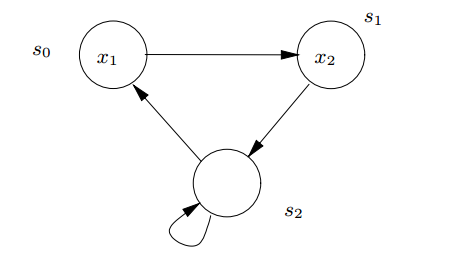
\includegraphics[scale=0.55]{symbolic_model_checking_example.PNG}
    \caption{A model}
    \label{fig:model_example}
\end{figure}
It consists of three states labelled $s_0, s_1,$ and $s_2$, and we consider two propositional variables, namely $x_1$ and $x_2$. 
If $S$ consitutes the whole state space, we can represent subsets of $S$ using Boolean formulae, as shown in the following table:\\

\begin{tabular}{ l | r }
  set of states & representation by boolean formula \\ \hline
$\emptyset $&   $\bot$ \\
$\{ s_0\}$ & $x_1 \land \lnot x_2 $\\
$\{ s_1\}$ & $ \lnot x_1 \land x_2 $\\
$\{ s_2\}$ & $\lnot x_1 \land \lnot x_2 $\\
$\{ s_0, s_ 1\}$ & $(x_1 \land \lnot x_2) \lor (\lnot x_1 \land x_2)  $\\
$\{ s_1, s_2\}$ & $(\lnot x_1 \land  x_2) \lor (\lnot x_1 \land\lnot x_2)$\\
$\{ s_0, s_2\}$ & $(x_1 \land \lnot x_2) \lor (\lnot x_1 \land\lnot x_2) $\\
$S$ & $(x_1 \land \lnot x_2) \lor (\lnot x_1 \land  x_2) \lor (\lnot x_1 \land\lnot x_2)$
\end{tabular}
\\
\\

Note that for this representation to be unambiguous, we must ensure that no two states satisfy the same set of Boolean variable. This can however be fixed by the addition of new Boolean variables which will be used to differenciate between the two (or more) ambiguous states.

\myparagraph{Symbolic Representation of the Transition Relation}

Note that the transition relation $\rightarrow$ of a model is a subset of $S \times S$. Taking two copies of our set of propositional variables, we can then associate a Boolean formula to the transition relation. In the example above, the transition relation $\rightarrow$ of the model is $\{(s_0, s_1), (s_1, s_2), (s_2, s_0), (s_2, s_2)\}$. 
Using our Boolean representations for $s_0, s_1$, and $s_2$, we compute the representation of $\rightarrow$ to be $$(\lnot x_1 \land \lnot x_2 \land \lnot x'_1 \land \lnot x'_2 ) \lor (\lnot x_1 \land \lnot x_2 \land x'_1 \land \lnot x'_2 ) \lor ( x_1 \land \lnot x_2 \land \lnot x'_1 \land  x'_2 ) \lor (\lnot x_1 \land x_2 \land \lnot x'_1 \land \lnot x'_2 )$$

[needs more details on the computation]


The next section explores the difference between different data structures and how they can be used to efficiently represent Boolean functions. 

\subsection{Representations of Boolean functions}

\subsubsection{Binary Decision Diagrams}

\myparagraph{Binary Decision Trees}

\myparagraph{Reduction Algorithm}

\myparagraph{Variable Ordering and Canonicity}

\subsubsection{A Knowledge Compilation Map}

In the field of Artificial Intelligence, Knowledge Compilation is a way of dealing with the computational intractability of various AI problems. The process consists in compiling a propositional model into a \textit{target compilation language} which is more convenient than the original model in a number of ways: 
\begin{itemize} 
\item The compactness of the compiled representation
\item The set of queries which are supported in polynomial time 
\item The computational complexity of Boolean operations on the representation 
\end{itemize}

According to \cite{knowledge_compilation_map}, all suitable target compilation languages are a subset of the Negation Normal Form (NNF):
\begin{definition}
A sentence in NNF is a rooted, direct acyclic graph (DAG) where each leaf node is labeled with true, false, $X$ or $\lnot X$ for a propositional variable $X$, and each internal node is labeled with $\land$ or $\lor$ and can have arbitrarily many children. 
\end{definition}  

In particular, BDDs and ROBDDs are both subsets of NNF. 


\subsubsection{Project Directions}

 In this project we aim to improve the efficiency of symbolic model checking by choosing a different target compilation language that the one implemented in most model checkers, namely BBDs. 
I considered several structures, including SDDs, d-DNNF and Trees-of-BDDs which are all subsets of NNF. The main criteria of choice were complexity of queries, canonicity, and usability for functions specific to model checking (e.g. \texttt{exists}), and after much consideration, SDDs seemed the most suitable to our usage.

The Sentential Decision Diagram was first introduced in 2011 at UCLA \cite{sdd_1} as a promising data structure for symbolic representation. With SDDs being relatively new, they have not yet been very much used for model checking and it is therefore very interesting to explore their possible use in this domain.
 In the next section we present a detailed description of SDDs. 


\subsection{SDDs}



\subsubsection{Preliminary Definitions}

To define SDDs formally we must start with some preliminary definitions. We use capital letters (e.g. \textbf{X}) to denote sets of Boolean variables and lower case letters (e.g. \textbf{x}) to denote their instantiations. 
\begin{definition} 
Let \textbf{X} be a set of variables. A \textit{Boolean function} $f$ maps an instantiation \textbf{x} to 0 or 1.
The \textit{conditioning} of $f$ on instantiation \textbf{z}, written $f|_{\textbf{z}}$ is the Boolean function obtained by setting variables in \textbf{Z} to their value in \textbf{z}. 
We say that a function $f$ \textit{essentially depends} on a variable x iff $f|_{\mbox{x}} \neq f|_{\lnot\mbox{x}}$, and we write $f(\textbf{X})$ if $f$ only essentially depends on variables in \textbf{X}.
\end{definition}

From now on we write $f(\textbf{X}, \textbf{Y})$ if $f(\textbf{Z})$, and \textbf{X}, \textbf{Y} are sets with $\textbf{X} \cup \textbf{Y} = \textbf{Z}$ and  
$\textbf{X} \cap \textbf{Y} = \emptyset$.
\begin{definition}
An (\textbf{X}, \textbf{Y})\textit{-decomposition} of a function $f(\textbf{X}, \textbf{Y})$ is a set of pairs $\{(p_1, s_1),...,(p_n, s_n)\}$ such that $$ f = (p_1(\textbf{X}) \land s_1(\textbf{Y})) \lor ... \lor (p_n(\textbf{X}) \land s_n(\textbf{Y}))$$
The decomposition is said to be \textit{strongly deterministic} on \textbf{X} if $p_i(\textbf{X}) \land p_j(\textbf{X}) = \bot$ for $i \neq j$. In this case, each ordered pair $(p_i, s_i)$ in the decomposition is called an \textit{element}, each $p_i$ a \textit{prime} and each $s_i$ a \textit{sub}.
\end{definition}

We now define the notion of \textbf{X}-partition as a more structured decomposition type. 
\begin{definition}
Let $\alpha = \{(p_1, s_1),...,(p_n, s_n)\}$ be an (\textbf{X}, \textbf{Y})-decomposition, and suppose $\alpha$ is strongly deterministic on \textbf{X}.
Then $\alpha$ is called an \textbf{X}-\textit{partition} iff its primes form a partition (i.e primes are pairwise mutually exclusive, each prime is consistent, and the disjunction of all primes is valid.)
We say that $\alpha$ is \textit{compressed} if $s_i \neq s_j$ for $i \neq j$.
\end{definition}

\begin{example} 
example
\end{example}

\begin{remark} Notice that $\bot$ can never be prime, and if $\top$ is prime then it is the only prime. Moreover primes determine subs, so two \textbf{X}-partitions are different iff they contain distinct primes.
\end{remark}

\begin{theorem}
Let $\circ$ be a Boolean operator and let $\{(p_1, s_1),...,(p_n, s_n)\}$ and $\{(q_1, r_1),...,(q_m, r_m)\}$  be \textbf{X}-partitions of Boolean functions $f(\textbf{X}, \textbf{Y})$ and $g(\textbf{X}, \textbf{Y})$ respectively. Then $$\{(p_i \land q_j, s_i \circ r_j) \mid  p_i \land q_j  \neq \bot \}$$ is an \textbf{X}-partition of $f \circ g$.
\end{theorem}
\begin{proof}
 proof
\end{proof}


\begin{theorem}
A function $f(\textbf{X}, \textbf{Y})$ has exaclty one compressed \textbf{X}-partition.
\end{theorem}
\begin{proof}
proof
\end{proof}

We now intoduce the notion of vtree, a key element in the construction of SDDs.

\begin{definition}
A \textit{vtree} for variables \textbf{X} is a full binary tree (i.e every node has exactly 0 or 2 children) whose leaves are in one-to-one correspondence with the variables in \textbf{X}. We will often not distinguish between a vtree node $v$ and the subtree rooted at $v$, and the left and right children of a node $v$ will be denoted $v^l$ and $v^r$, respectively.
\end{definition}

\begin{example}
example
\end{example}


Note that a vtree on \textbf{X} is stronger than a total order of the variables in \textbf{X}. Example \ref{test} shows two distinct vtrees which induce the same variable order. 

Now, let $f(\textbf{X})$ be a Boolean function and let $v$ be a vtree for \textbf{X}. We can construct an SDD for $f$ using a recursive algorithm, as follows.

 We first notice that variables in \textbf{X} are split into two disjoint sets, namely the variables in $v^l$ (say, \textbf{Y}) and the variables in $v^r$ (say, \textbf{Z}). Now, let $\alpha =  \{(p_1, s_1),...,(p_n, s_n)\}$ be a \textbf{Y}-partition of $f(\textbf{Y}, \textbf{Z})$. We apply this decomposition again to each prime 

[...] describe more
\subsubsection{Syntax and Semantics of SDDs}


\begin{definition} (Syntax)
Let $v$ be a vtree. $\alpha$ is an SDD that respects $v$ iff: 
\begin{itemize} 
\item $\alpha = \top$ or $\alpha = \bot$
\item $\alpha = X$ or $\alpha = \lnot X$, and $v$ is a leaf with variable $X$
\item $v$ is internal, and $\alpha$ is a partition  $\{(p_1, s_1), ..., (p_n, s_n)\}$ such that for all $i$, $p_i$ is an SDD that respects $v^l$ and $s_i$ is an SDD that respects $v^r$.
\end{itemize}
In the first two cases we say that $\alpha$ is \textit{terminal}, and in the third case $\alpha$ is called a \textit{decomposition}. For SDDs $\alpha$ and $\beta$, we write $\alpha = \beta$ iff they are \textit{syntactically equal}.
\end{definition}

\begin{definition} (Semantics)
Let $\alpha$ be an SDD. We use $\langle . \rangle$ to denote the mapping from SDDs to Boolean functions, and we define it inductively as follows: 
\begin{itemize} 
\item $\langle \top \rangle = \top$ and  $\langle \bot \rangle = \bot$
\item $\langle X \rangle = X$ and $\langle \lnot X \rangle = \lnot X$, for all variables $X$
\item $\langle\{(p_1, s_1), ..., (p_n, s_n)\}\rangle = \bigvee_{i = 1}^n \langle p_i \rangle \land \langle s_i \rangle  $
\end{itemize}
We say two SDDs $\alpha$ and $\beta$ are \textit{equivalent} (written $\alpha \equiv \beta$) if $\langle \alpha \rangle = \langle \beta \rangle$.

\end{definition}


\subsubsection{Construction of SDDs}



\subsubsection{Canonicity of SDDs} 

It is obvious that if SDDs $\alpha$ and $\beta$ are equal, then they are equivalent. We would however like 
to impose conditions on the construction of $\alpha$ and $\beta$  so that $\alpha \equiv \beta \Rightarrow \alpha = \beta$.
We begin with a few definitions and lemmas.

\begin{definition}
Let $f$ be a non-trivial Boolean function. We say $f$ \textit{essentially depends} on vtree node $v$ if $v$ is a deepest node that includes all variables that $f$ essentially depends on. 
\end{definition}

\begin{lemma}
A non-trivial function essentially depends on exactly one vtree node.
\end{lemma} 

\begin{proof} 

\end{proof}
 
\begin{definition}
An SDD is \textit{compressed} iff all its decompositions are compressed. It is \textit{trimmed} iff it does not have decompositions of the form $\{(\top, \alpha)\}$ or $\{(\alpha, \top), (\lnot\alpha, \bot)\}$ for some SDD $\alpha$.
\end{definition}

An SDD can be trimmed by traversing it bottom-up and replacing decompositions of the form  $\{(\top, \alpha)\}$ or $\{(\alpha, \top), (\lnot\alpha, \bot)\}$ by $\alpha$.

\begin{theorem} 
Let $\alpha$ and $\beta$ be compressed and trimmed SDDs. Then $$\alpha = \beta \Leftrightarrow \alpha \equiv \beta$$
\end{theorem}

\begin{proof}
by induction
\end{proof}

\subsubsection{SDD Operations}

The \texttt{apply} algorithm to compose SDDs $\alpha$ and $\beta$ using a Boolean operator takes time $O(|\alpha||\beta|)$ provided both SDDs 
are normalised. See \cite{sdd_1} for details of the algorithm.

The \texttt{exists} algorithm is the implementation of the $\exists X$ operator on function $f$ for variable $X$. Recall $$\exists X f = f[0/X] \lor f[1/X]$$
This can be implemented using the \texttt{restrict} algorithm which returns the conditioning $f|_{\mbox{x}}$ for an instantiation x of $X$.  
 
\subsubsection{Symbolic Model Checking with SDDs}

\myparagraph{Computing the Reachable State Space}

Let $X \subseteq S$ be a set of states. We define $T(X)$ to be the set of states reachable from a state in $X$ in one step, i.e. $$T(X) = \{ s \mid \exists s' \in X\mbox{ such that }s' \rightarrow s \}$$

Suppose $S_X$ is an SDD for the set $X$, and let $S_{\rightarrow}$ be the SDD representation of the transition relation of the model. 
Then the SDD for $T(X$) can be computed as follows: 
\begin{enumerate} 
\item Compute $\texttt{exists}(\hat{x}, \texttt{apply}(\land, S_X, S_{\rightarrow}) )$ (where $\hat{x}$ represents $(x_1, ..., x_n )$)
\item ``Un-prime'' all variables in the resulting SDD.
\end{enumerate}

We can now compute the whole reachable state space, starting from the set of initial states $X_0$ and iteratively applying $T$. This is described in the pseudo-code below:

\begin{lstlisting}[mathescape]
Reachable State Space:
X = X$_{\mbox{0}}$
	while (X  $\neq$ Y) 
	Y = X
	X = X $\cup$ T(X)
return X
\end{lstlisting}

\myparagraph{Labelling of Formulae}

The labelling algorithm as presented above uses the functions 
$\pre_{\exists}$ and $\pre_{\forall}$. 

Notice that if $S$ is the entire state space, and $X \subseteq S$, we have that $\pre_{\forall}(X) = S - \pre_{\exists}(S - X)$ and therefore we only need to be able to compute $\pre_{\exists}$ on SDDs.

Suppose $S_X$ is an SDD for the set $X$, and let $S_{\rightarrow}$ be the SDD representation of the transition relation of the model. 
Then the SDD for $\pre_{\exists}(X)$  can be computed as follows: 
\begin{enumerate} 
\item Rename all variables in $S_X$ to their primed version. Call the resulting SDD $S_{X'}$.
\item Compute $\texttt{exists}(\hat{x}', \texttt{apply}(\land, S_{\rightarrow},  S_{X'}) )$ (where $\hat{x}'$ represents $(x_1', ..., x_n ')$)
\end{enumerate}



\section{Implementation}

The ultimate objective of the project is to implement a model checker which is based on SDDs. As the implementation of a full model checker from scratch would be too big a task for a project of this scale, I decided to re-use parts of an existing model checker, MCMAS. 

\subsection{MCMAS}
 
MCMAS (Model Checker for Multi-Agent Systems) is an open-source OBDD-based symbolic model checker tailored to the verification of Multi-Agent Systems. \cite{MCMAS_website} It is primarily developed at Imperial College London.

Users can input a description of a MAS using the Interpreted Systems Programming Language (ISPL), whose syntax is very much inspired from the formal definition of interpreted systems (see Section ?). MCMAS allows the verification of specifications including, among others, CTL operators and epistemic operators.

\subsubsection{CUDD}

As an OBDD-based model checker, MCMAS relies on an external package for creating and manipulating OBDDs. 
CUDD, an open-source package developed at the University of Colorado, provides this functionality. \cite{CUDD_website}

In this project we aim to improve the efficiency of MCMAS by replacing CUDD with an appropriate SDD package.

\subsubsection{Sofware Architecture}

 
 \subsubsection{Eclipse Interface}

 MCMAS offerss a graphical user interface (GUI) built as an Eclipse plug-in. The plug-in provides functionality including an ISPL syntax checker, an interactive execution mode and \emph{counterexample display}. 
 

\subsection{Tools}

\subsubsection{The SDD package} 

\cite{SDD_website}
``The SDD Package'' is a C library providing functionality for manipulating SDDs. It allows for the manual constuction of SDDs from elementary SDDs, and provides helpful optimisation functionalities.

\myparagraph{Queries and Transformations}

This library provides an API for quering and applying operations on SDDs. In addition to the usual Boolean operators, it offers built-in functions for \texttt{exists} and \texttt{forall} which are particularly relevant in the case of model checking. 

\myparagraph{Vtree Optimization}

As explained in the previous sections, the size of an SDD can vary a lot depending on the vtree it is based on. Hence the problem of optimising an SDD comes down to finding an appropriate vtree, and to that algorithms have been developed involving going through the space of vtrees in a specific order. The SDD package provides the implementation for a minimisation algorithm, which I will have to investigate in order for the performance of my model checker to be as good as possible.

\myparagraph{DNF/CNF to SDD Compiler}

Included in the SDD library is an FNF-to-SDD Compiler (FNF = Flat Normal Form, CNF or DNF). This feature will allow me to encode propositional databases into SDDs in a very easy way. 

\myparagraph{Garbage Collection}

In the library also features an optimised garbage collector. Since the construction of an SDD generates a lot of ``garbage SDDs'', it is important that I use this in my implementation in order to maximise the speed increase. 

\myparagraph{Graphics}

The package provides the option to ``export as dot files'' the output of SDD computations, which offers a convenient way of drawing graphs and diagrams, in particular vtrees and SDDs.
This could potentially be used if I need to provide a user-friendly interface to interact with the SDD package. 


\subsubsection{Results Measurements}

`

\subsubsection{Development Environment}

\myparagraph{Eclipse}

I chose to use Eclipse for C/C++ development, for two main reasons. 
The first one is that I am most used to working with this IDE, and it offers a number of different plugins which can be used to facilitate tasks such as measuring performance and version control. 
The second reason I am using Eclipse is because of the MCMAS Eclipse interface described above, which would require me to use Eclipse if I was to extend the interface to SDDs. 

\myparagraph{Version Control}

For a project of this scale, it would be unreasonable not to use a version control system. Such a system makes it easier to revert back in case of an unwanted change, or maintain several versions of the same code.  For this project, I have chosen to use Git since I have previous experience with it and the system integrates well within Eclipse. 


\subsection{Project Plan}

\subsubsection{Main Deliverables}

Through this project I aim to produce:
\begin{itemize}
\item A detailed theory of Symbolic Model Checking and SDDs
\item A symbolic model checker for multi-agent systems, based on SDDs
\item An user interface allowing the user to investigate the ``SDD stats'' of their specification as well as try different optimisation options
\end{itemize}

In order to do this, I will first need to review all Model Checking concepts and make sure I am very comfortable with the topics. I will need to do some background reading on Knowledge Compilation and representation of Boolean functions, to be able to understand perfectly the ideas surrounding SDDs.

Next I will have to become familiar with the implementation of MCMAS and the way the CUDD system is integrated. I will have to get used to the functions proposed by the SDD package described above, and probably go through a few different examples in order to really undersand the way SDDs should be manipulated.

Finally I plan to thoroughly implement a new version of MCMAS which is based on the SDD package.
I will have to leave enough time at the end of the project for extensive testing (to verify the correctness of my software, but mainly to test the performance of a model checker with SDDs) and to establish a comparison between BDDs and SDDs in terms of performance in model checking. 

\subsubsection{Time Plan}

[insert Gantt Chart]

\subsubsection{Possible Extensions}

\myparagraph{The MCMAS Eclipse interface}

One possible feature that I will add to my project if I have time is an adaptation of the MCMAS Eclipse interface.

\myparagraph{Other data structures?}

I would also really like to explore the application to model checking of different, more recent Boolean structures, some of which have been described as promising in terms of size and query performance. Obviously this would consist in a whole other project, but it would be interesting to start investigating further.

\clearpage
\section{Evaluation}

At the end of the implementation, I will need to evaluate the performance of the model checker in order to establish a detailed comparison with the original MCMAS based on BDDs.
To this aim I intend to try the new model checker on a variety of different examples of MAS, including: 
\begin{itemize}
\item The bit transmission problem,
\item The muddy children,
\item The philosophers' dinner
\end{itemize}
and others whose model may present different characteristics. 

\section{Conclusion}

This project should provide enough information to know in which case (if any) it might be more interesting to use SDDs than BDDs.


\begin{thebibliography}{9}

\bibitem{sdd_1}
A. Darwiche,\emph{ SDD: A New Canonical Representation of Propositional Knowledge Bases}, 2011

\bibitem{knowledge_compilation_map}
  A. Darwiche, P. Marquis,
  \emph{A Knowledge Compilation Map}, 2002.

\bibitem{logic_in_computer_science}
 M. Huth, M. Ryan, 
\emph{Logic in Computer Science},
Cambridge University Press, 2004.

\bibitem{MCMAS_website} MCMAS webpage, http://vas.doc.ic.ac.uk/software/mcmas/

\bibitem{CUDD_website} CUDD Package webpage, http://vlsi.colorado.edu/~fabio/CUDD/

\bibitem{SDD_website} SDD Package webpage, http://reasoning.cs.ucla.edu/sdd/

\bibitem{notes} A. Lomuscio, Software Engineering: Software Verifications Lecture Notes (as taught in 2012-13)


\end{thebibliography}


\end{document}